\chapter{Medical Imaging and Image Segmentation}
\label{chap:2}
%

The first steps in image-based modeling and simulation involve \textit{image acquisition}, \textit{image processing}, and \textit{image segmentation}. Several techniques are available to produce three-dimensional image data of an anatomical region of interest and are reviewed herein. State-of-the art image processing and image segmentation approaches are also summarized.

%%%%%%%%%%%%%%%%%%%%%%%%%%%%%%%%%%%%%%%%%%%%%%%
%%%%%%%%%%%%%%%%%%%%%%%%%%%%%%%%%%%%%%%%%%%%%%%
\section{Medical Imaging Approaches}
\label{Medical Imaging Approaches}

Medical imaging is the process of generating discrete image representations of biological tissues. Of the many imaging modalities found in clinical and research settings, the most prevalent are \textit{magnetic resonance imaging} (MRI) and \textit{x-ray computed tomography} (CT). Both approaches are \textit{tomographic} in that they produce a series of two-dimensional images representing thin slices of the region of interest, that are subsequently combined to produce a three-dimensional volume representation \cite{larobina_murino_2014}. The data measured during acquisition are different for each modality, and thus the appropriate imaging technique for a particular use depends on the tissues of interest. Images typically have on the order of millimeter or sub-millimeter voxel resolution. The basic physics of MRI and CT technologies are discussed. Several other imaging techniques exist - some of which provide more information than do MRI and CT - and are briefly presented in this section as well. Finally, typical data storage approaches and file formats are discussed.

\subsection{Magnetic Resonance Imaging}
\label{Magnetic Resonance Imaging}

Magnetic resonance imaging (MRI) is the process of generating images via the physical phenomenon of nuclear magnetic resonance (NMR), in which nuclei in a magnetic field absorb and re-emit electromagnetic radiation at their \textit{resonant frequency}~\cite{NMR}. Gradients in the magnetic field are used to encode the response at different locations in the region. MRI provides excellent soft tissue contrast, for tissues such as articular cartilage, bone marrow, muscle, ligaments, and gray and white matter in the brain. Unlike CT, it does not use any harmful ionizing radiation~\cite{waldman_campbell}. A brief description of the basic physics in acquiring an MRI follows.

A strong external magnet generates a magnetic field $B_0\bm{e}_z$ that is constant in time and space, within which the patient or object is placed. The $z$ direction corresponds to the image slice thickness direction. For most clinical applications, the strength of this field is 1.5 Tesla or 3 Tesla. For reference, a 3 T magnetic field is roughly 60,000 times stronger than Earth's magnetic field. Shim coils are used to correct or ``shim'' the magnetic field so as to ensure good field homogeneity, which results in a high-quality signal~\cite{jacobs_2007}. Dipole moments in the nuclei of certain elements align either in parallel or anti-parallel to the direction of the applied magnetic field, similarly to how a bar magnet orients itself in the presence of an external magnetic field~\cite{hendrick_1994}. The parallel orientation provides a slightly lower energy state than that for the anti-parallel orientation, and thus the dipole moments prefer to align with the direction of the applied magnetic field. Prior to applying the external magnetic field, the random orientation of the nuclear magnetic dipoles in the tissue produce a zero net magnetization, but following the imposition of a static magnetic field, a net magnetization of tissue $M_0\bm{e}_z$ is produced from the preferential alignment of dipoles~(see~\figref{mr1}).

Due to the prevalence of hydrogen in biological tissues - most notably in water and fat - MR imaging is typically based on the behavior of the nuclear magnetic dipole of hydrogen.

\begin{figure}[ht]
\centering
\subfigure[]{%
		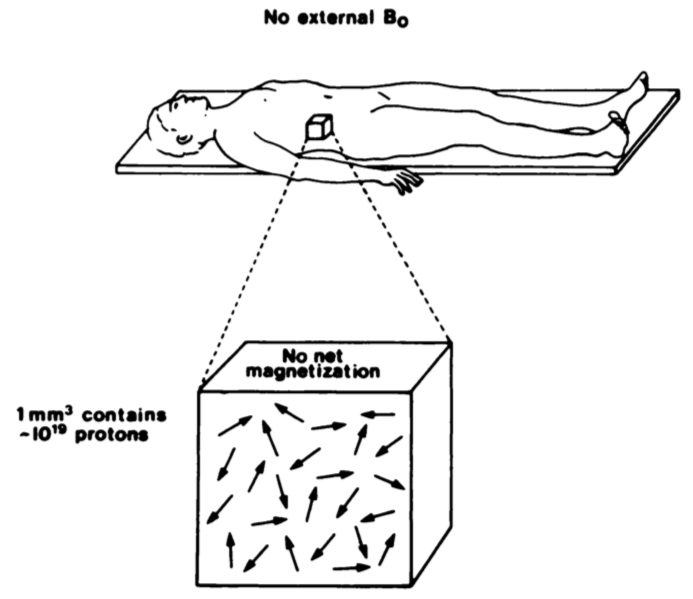
\includegraphics[scale=0.25]{media/0-imaging/mr1a.png}
\label{fig:mr11}}
\subfigure[]{%
		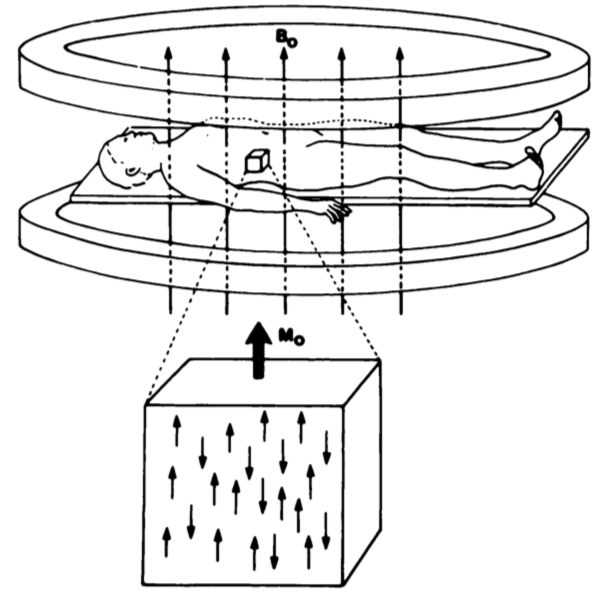
\includegraphics[scale=0.25]{media/0-imaging/mr1b.png}
\label{fig:mr12}}
%
\caption{Net magnetization $M_0$ in a voxel of tissue (a) prior to, and (b) following the application of a static external magnetic field $B_0$~\cite{hendrick_1994}}
\label{fig:mr1}
\end{figure}

If the net magnetization is perturbed from pointing in the same direction of a magnetic field $B\bm{e}_z$, the new magnetization $M$ \textit{precesses} about the $z$ axis. The \textit{precessional frequency} or \textit{Larmor frequency} $\omega$ is defined by the relationship:
\begin{equation}
\omega = \gamma B
\end{equation}
where the constant $\gamma$ is the \textit{gyromagnetic ratio}, which is 42.6 MHz/T for hydrogen. In MR imaging, the net magnetization is tipped away from the direction of $B_0$ by applying a radio-frequency (RF) pulse that oscillates exactly at the Larmor frequency. The precessing transverse magnetization produces a changing magnetic field, which induces an electric current and is recorded by the receiver coil~(see~\figref{mr2}).

\begin{figure}[ht]
\centering
\subfigure[]{%
		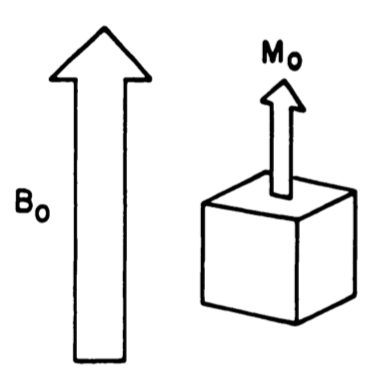
\includegraphics[scale=0.25]{media/0-imaging/mr2a.png}
\label{fig:mr21}}
\subfigure[]{%
		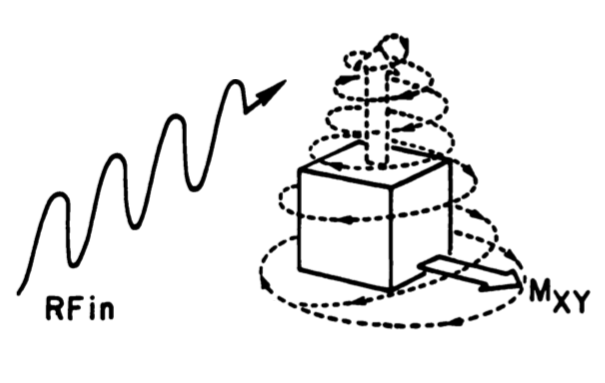
\includegraphics[scale=0.25]{media/0-imaging/mr2b.png}
\label{fig:mr22}}
\subfigure[]{%
		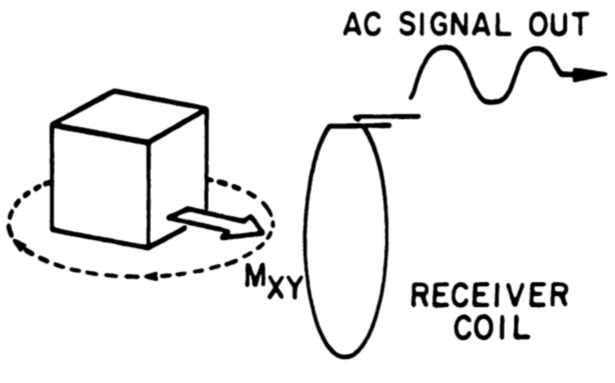
\includegraphics[scale=0.25]{media/0-imaging/mr2c.png}
\label{fig:mr23}}
%
\caption{Basic premise of MRI: (a) An external magnetic field $B_0$ causes a net magnetization $M_0$ of a voxel of tissue pointing in the same direction as the applied field, (b) an RF pulse applied at the precessional frequency of hydrogen causes the magnetization vector to tilt from a longitudinal direction into the transverse plane, and (c) the amplitude, frequency, and phase of the time-varying signal from the transverse magnetization $M_{xy}$ is recorded~\cite{hendrick_1994}}
\label{fig:mr2}
\end{figure}

In order for the receiver coil to distinguish between different locations in the object, \textit{spatial localization} of the MR signal is achieved by applying linear magnetic field gradients in each of the three spatial directions. Namely, the new spatially varying magnetic field $B(\bm{x})\bm{e}_z$ (still pointing in $z$ direction), following the imposition of magnetic gradients, becomes:
\begin{equation}
B(\bm{x}) = B_0 + \bm{G}(t) \cdot \bm{x}
\label{eqn:gradient}
\end{equation}
Multiplying \eqnref{gradient} by $\gamma$ yields:
\begin{equation}
\omega(\bm{x}) = \omega_0 + \bm{G}(t) \cdot \bm{x}
\label{eqn:freq}
\end{equation}
Thus, each RF signal oscillates at the appropriate frequency to excite and record information for each unique voxel in the image.

The magnetic field gradient $\bm{G}(t) = (G_x, G_y, G_z)$ is applied in stages.. Specifically, the magnetic gradient $G_z$ and corresponding RF pulse are first turned on to excite a particular slice (or section) of tissue. Excitation here refers to the perturbation of the net magnetization away from the $z$ direction into the transverse plane. $G_z$ is referred to as the \textit{slice-selection gradient}. The resolution of the image in the $z$ direction may be increased by reducing the bandwidth of the RF pulse or increasing the strength of the applied gradient. To resolve the selected section into voxels, gradients are applied separately in each of the two in-plane directions $x$ and $y$. The magnetic gradient $G_y$ is applied and removed following signal excitation. While turned on, the gradient causes strips of hydrogen nuclei within the slice to precess at different speeds for a brief period of time. When the gradient is turned off, different strips maintain the same precessional frequency within the same slice, but a fixed phase difference now exists among them. $G_y$ is referred to as the \textit{phase-encoding gradient}. Finally, the magnetic gradient $G_x$ alters the resonant frequency along the $x$ direction. It separates each strip into voxels, each voxel resonating at a different frequency. $G_x$ is applied at the time of signal measurement and is referred to as the  \textit{frequency-encoding gradient} or the \textit{readout gradient}. The resolution of the in-plane image may be improved by increasing the number of pulse sequence acquisitions and subsequent measurements. See \figref{mr3} for a visual representation of these steps.

\begin{figure}[ht]
\centering
\subfigure[]{%
		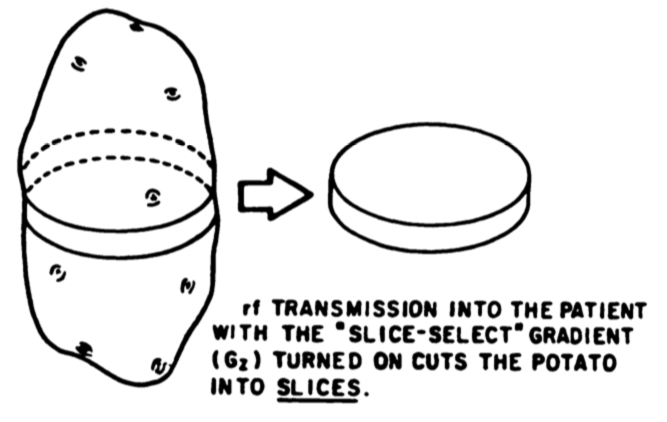
\includegraphics[scale=0.21]{media/0-imaging/mr3a.png}
\label{fig:mr31}}
\subfigure[]{%
		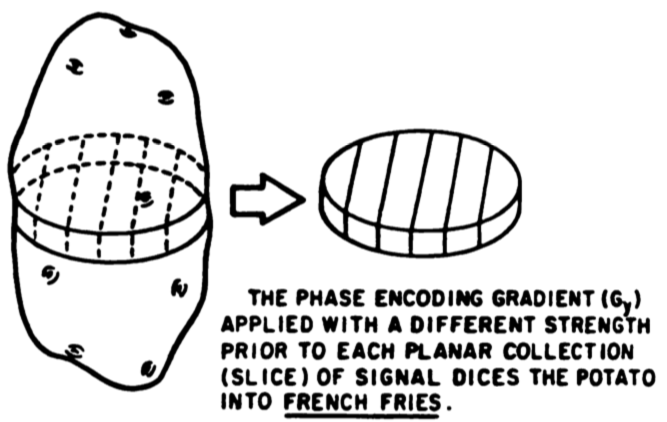
\includegraphics[scale=0.21]{media/0-imaging/mr3b.png}
\label{fig:mr32}}
\subfigure[]{%
		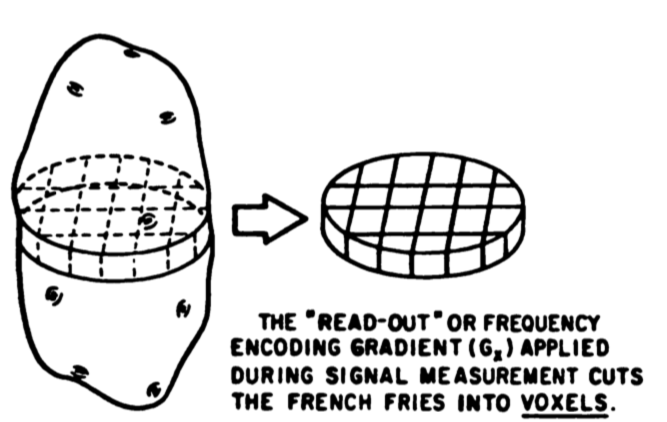
\includegraphics[scale=0.21]{media/0-imaging/mr3c.png}
\label{fig:mr33}}
%
\caption{Visual representation spatial localization based on successive application of magnetic gradients: (a) slice-selection gradient, (b) phase-encoding gradient, and (c) frequency-encoding gradient~\cite{hendrick_1994}}
\label{fig:mr3}
\end{figure}

MRI signal intensity at a particular voxel typically depends on the proton density of the tissue (via the strength of the net magnetization $M_0$) and two \textit{relaxation times} T1 and T2 corresponding to the exponential decay of the perturbed net magnetization back to its original state following an RF pulse. Following a typical $90^{\circ}$ RF pulse, which maximizes the transverse magnetization $M_{xy}$, the relaxation times are defined by the following relationships:
\begin{align}
M(t) &= M_0(1 - e^{(-t/T1)}) \\
M_{xy}(t) &= M_{xy}e^{(-t/T2)}
\end{align}
The \textit{T1 recovery time} (also known as the \textit{spin-lattice} or \textit{longitudinal recovery time}) corresponds to the recovery of the longitudinal magnetization $M_0$. This reorientation is caused by the transfer of energy from the excited magnetic dipoles to the surrounding lattice of molecules. The \textit{T2 recovery time}  (also known as the \textit{transverse} or \textit{spin-spin recovery time}) corresponds to neighboring precessing magnetic dipoles \textit{dephasing}. Dephasing occurs because as the transverse magnetization decays, slightly different magnetic environments exist for neighboring hydrogen nuclei in different regions of a particular voxel.

Tissue contrasts are created based on the strength and timing of the RF pulse; this is known as the \textit{MR sequence}. The parameters in MR pulse sequences weight the influence of proton density, T1, and T2 differently in the final MR signal. The most basic MR sequences are \textit{proton density} (PD), \textit{T1-weighted} (T1W), and \textit{T2-weighted} (T2W), each of which provide different tissue contrasts. The choice of an MR sequence will depend on the tissues and applications of interest of the scan. A number of references are available for a more detailed description of T1, T2, the parameters of an MR sequence, and their relationship in creating tissue contrast~\cite{nishimura_2010, brown_semelka_2003, webb_2003} .

For each voxel in a slice, the amplitude, phase, and frequency of the time-varying MR signal is recorded by the receiver coil in the \textit{frequency domain}, or what is known as \textit{k-space}. For each slice, the frequency domain is converted to the spatial domain (i.e., the two-dimensional image for a particular slice) via 2D inverse Fourier transform. The k-space of an image can be modified to identify artifacts, remove noise, and enhance contrast~\cite{imaios}. Please refer to the references in this section for more detail on k-space and its manipulations. Finally, each 2D image is combined to form a 3D grayscale image corresponding to the object scanned. The intensity at each voxel in the three-dimensional rectilinear grid is a weighted proton density. The value at each voxel can represent many different units of measure depending on the pulse sequence~\cite{beek_hoffman_2008}.

\subsection{X-Ray Computed Tomography}
\label{X-Ray Computed Tomography}

X-ray computed tomography (CT) is the process of generating images via the emission of an x-ray beam source, and subsequently detecting the \textit{attenuation} of the x-ray beam through the various tissues in the patient or object. CT provides excellent contrast for bone, but is less suitable in measuring soft tissue contrast compared to MRI. Acquisition times are typically less than those for MRI, image resolutions are typically higher~\cite{pomeranz_2007}, and ionizing radiation from the x-ray beam must also be carefully considered. The basic principles of image acquisition via CT technology ensue.

In CT, an x-ray beam source is emitted through the plane of a finite thickness cross section of the object~\cite{mahesh_2002}. The mean attenuation of the x-ray beam through each voxel within the slice is measured by a detector on the other side of the object. The attenuation data is reconstructed into a digital two-dimensional image. Once again, the set of 2D images is stacked together to form a 3D image representation of the region being scanned.

Attenuation measures the amount by which x-ray radiation is reduced in passing through a material. For an inhomogeneous material, the attenuation along a particular ray line is expressed in the following relationship:
\begin{equation}
I= I_0e^{-\int\limits_{0}^{L}f(x,y) ds}
\label{eqn:init}
\end{equation}
where $I_0$ is the x-ray intensity emitted in front of the object, $I$ is the x-ray intensity received behind the object, $f(x,y)$ is the linear attenuation coefficient for the material at location $(x,y)$, $L$ is the length over which the beam travels through the material, and $ds$ is the length of a differential cut along the ray. The variable $s$ is parameterized as a function of $x$ and $y$. In first generation CT machines, for a particular slice, the x-ray tube and detector were rigidly translated together across the subject as x-ray beams were emitted and recorded~(see~\figref{ct1}).

\begin{figure}[ht]
\centering
		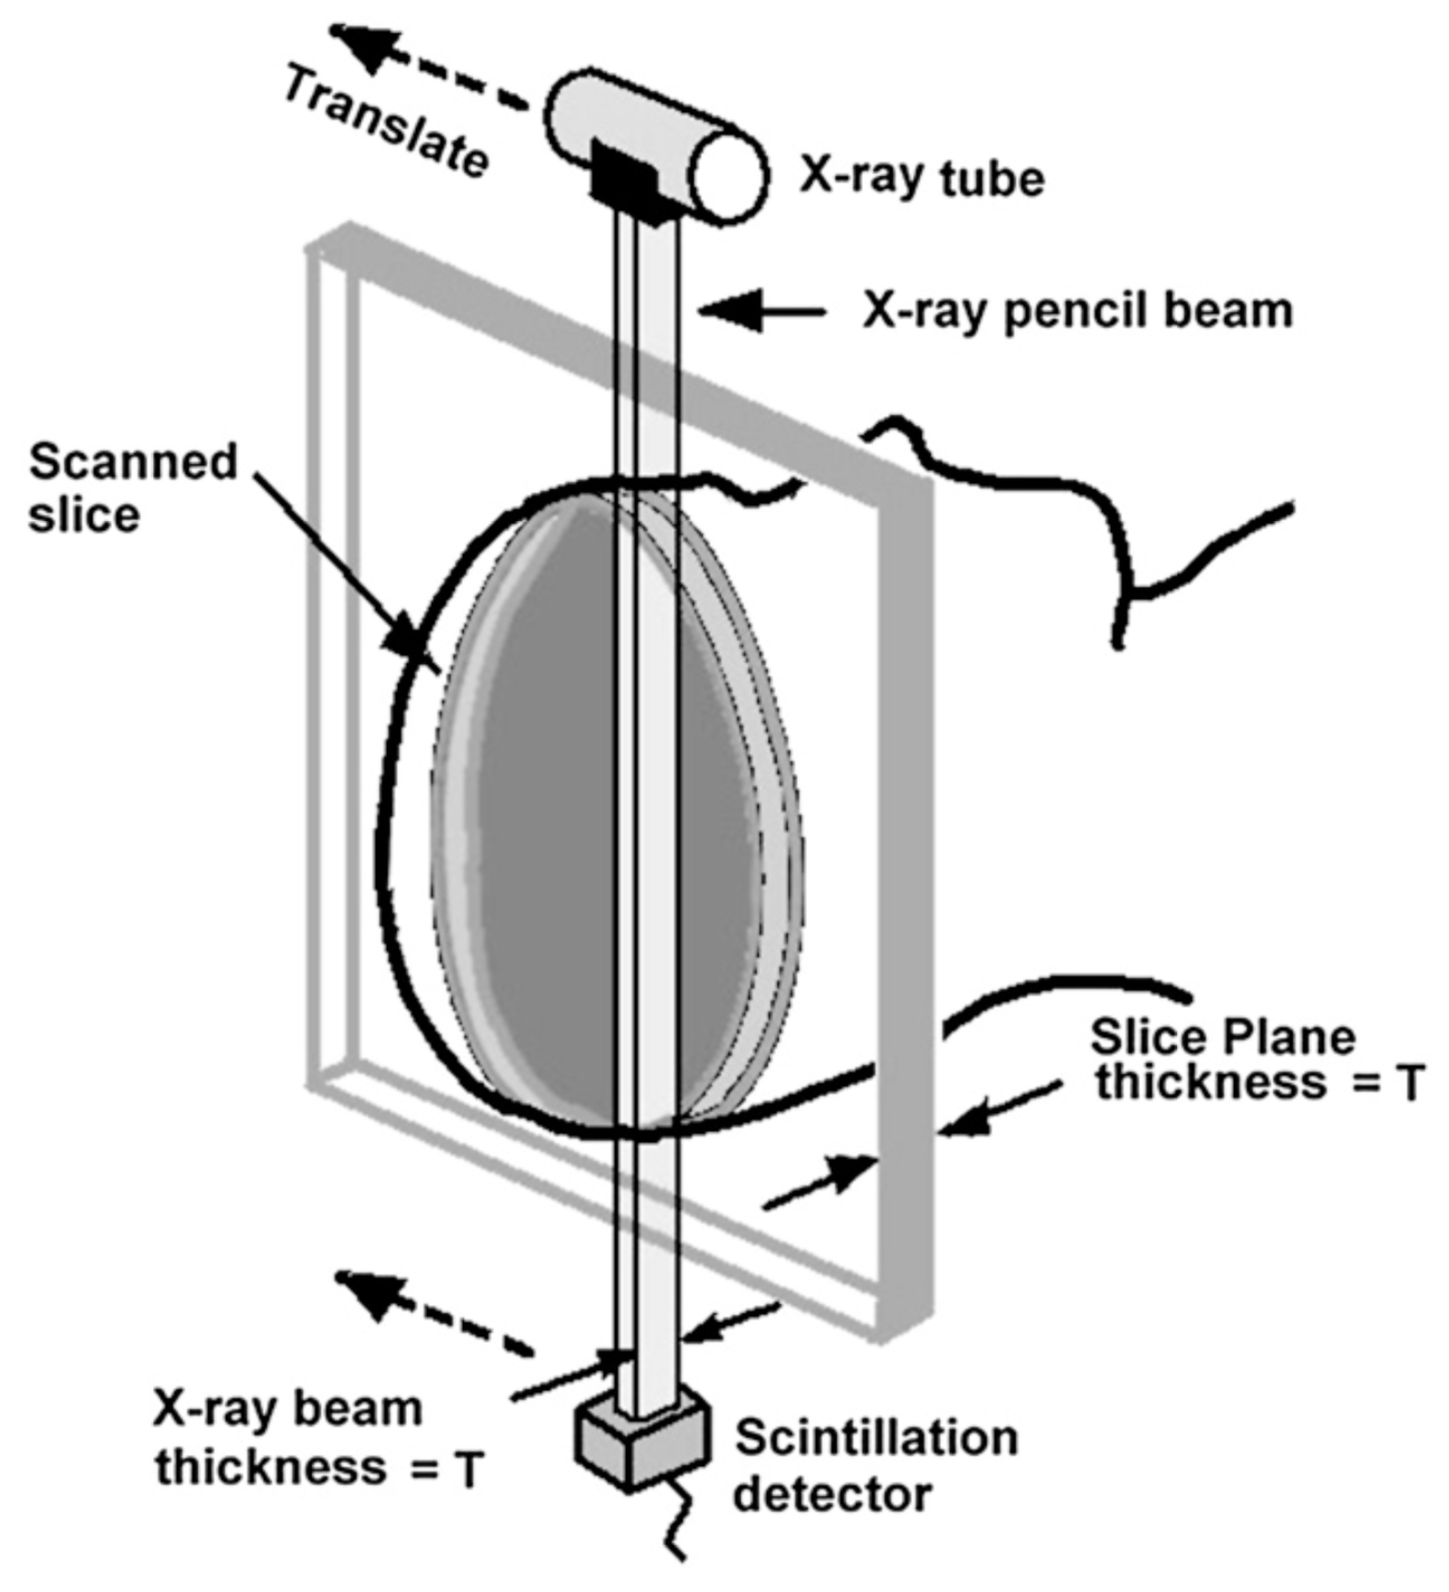
\includegraphics[scale=0.3]{media/0-imaging/ct1.png}
%
\caption{CT arrangement for linear transverse scanning motion of x-ray tube and detector. ~\cite{goldman_2007}}
\label{fig:ct1}
\end{figure}

The x-ray beam path is referred to as a \textit{ray}. The set of rays and measurements made during the translation is known as a \textit{view}. Several hundred rays are measured in a particular view. The assembly is then rotated about the axis perpendicular to the slice plane by a small increment and a new view is captured. Over 1000 views are captured as the assembly is rotated through 360$^{\circ}$. Thus, the total number of measurements for a particular slice is the number of rays per view multiplied by the number of views, and is on the order of one million measurements per slice in modern CT machines~(see~\figref{ct2}).

\begin{figure}[ht]
\centering
		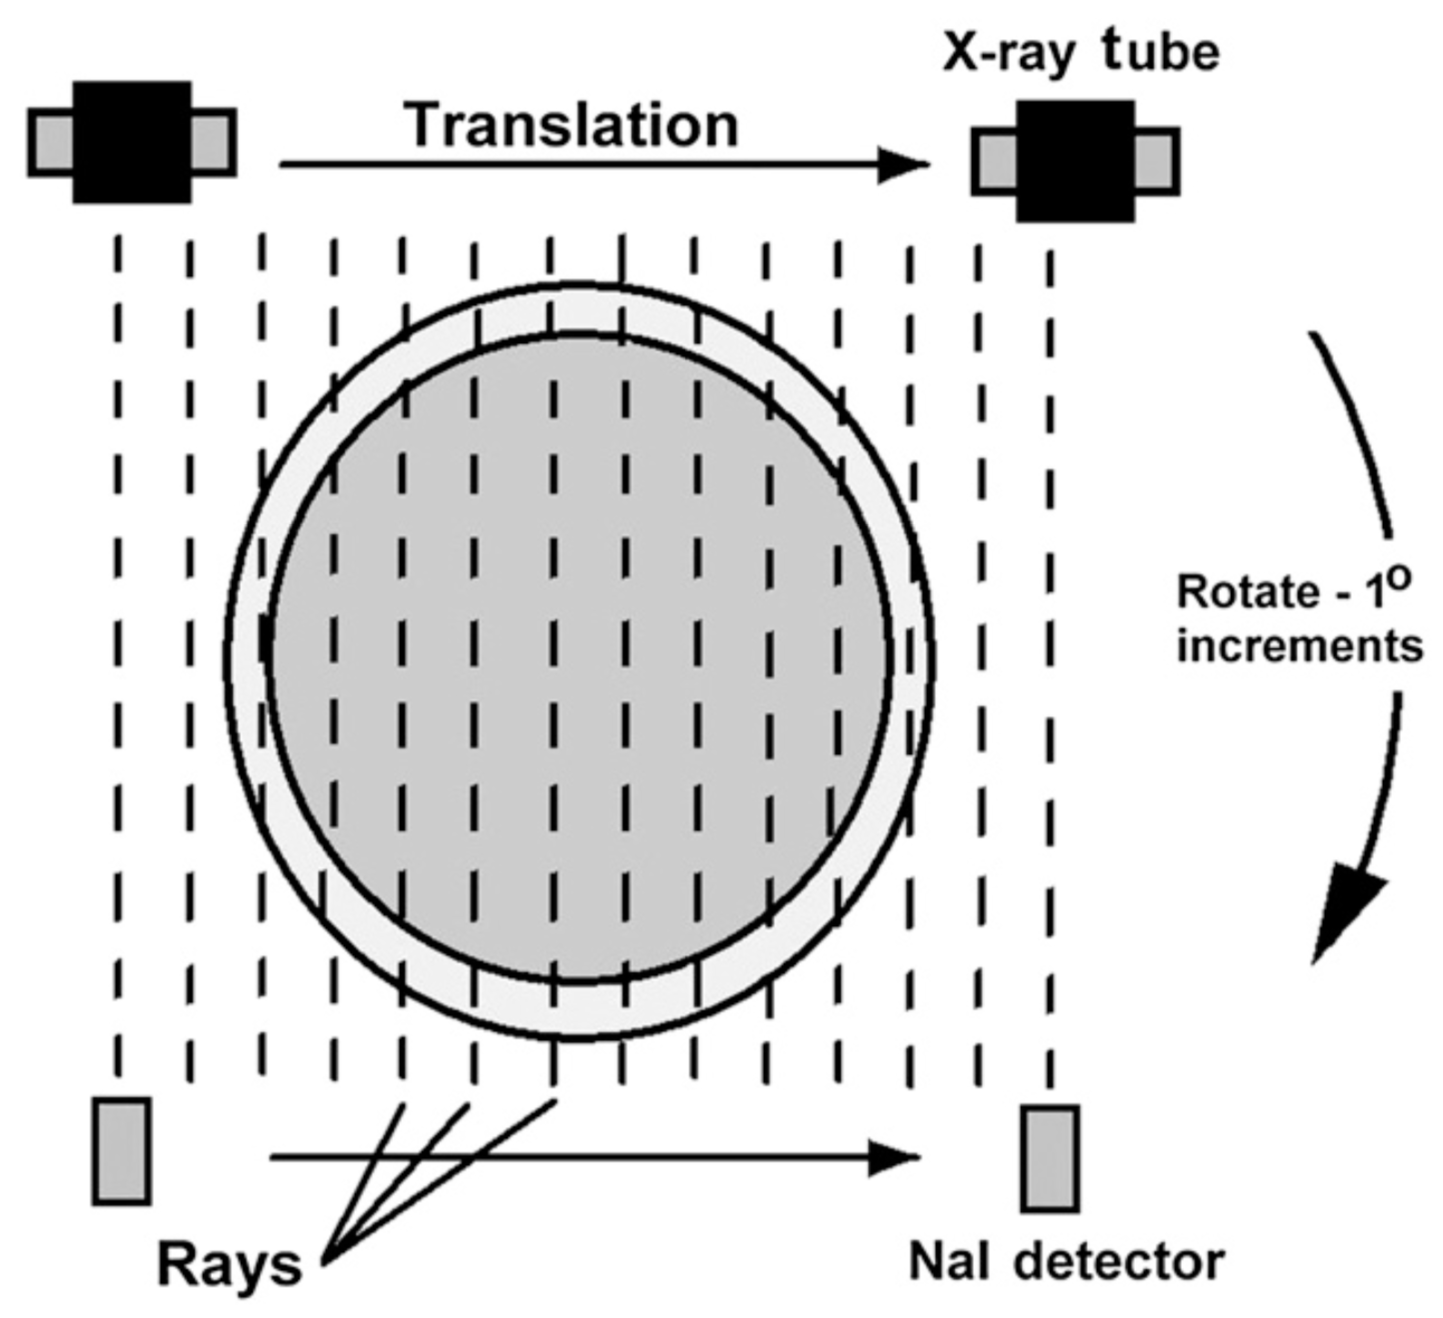
\includegraphics[scale=0.3]{media/0-imaging/ct2.png}
%
\caption{Measurement procedure for first-generation CT. Rays are emitted from the x-ray tube and the attenuated radiation is measured by the detector. The assembly is translated in increments to cover the span of the slice. The process is repeated as the assembly is rotated in increments through 360$^{\circ}$~\cite{goldman_2007}}
\label{fig:ct2}
\end{figure}

\textit{Image reconstruction} is the process of deriving the average attenuation coefficient values $f$ for each voxel in a slice from the attenuation measurements made by the x-ray detector. Attenuation increases with the density and atomic number of the tissues in the voxel. Rearranging~\eqnref{init} yields:
\begin{equation}
p(\xi, \theta) = -\ln(I/I_0) = \int\limits_{0}^{L}f(x,y) ds
\end{equation}
The function $p(\xi,\theta)$ is known as the \textit{Radon transform} of the attenuation function $f(x,y)$. The angle $\theta$ corresponds to the angle of rotation of the view, and $\xi$ corresponds to the position along the measured x-ray projection~(see~\figref{ct3}).

\begin{figure}[ht]
\centering
		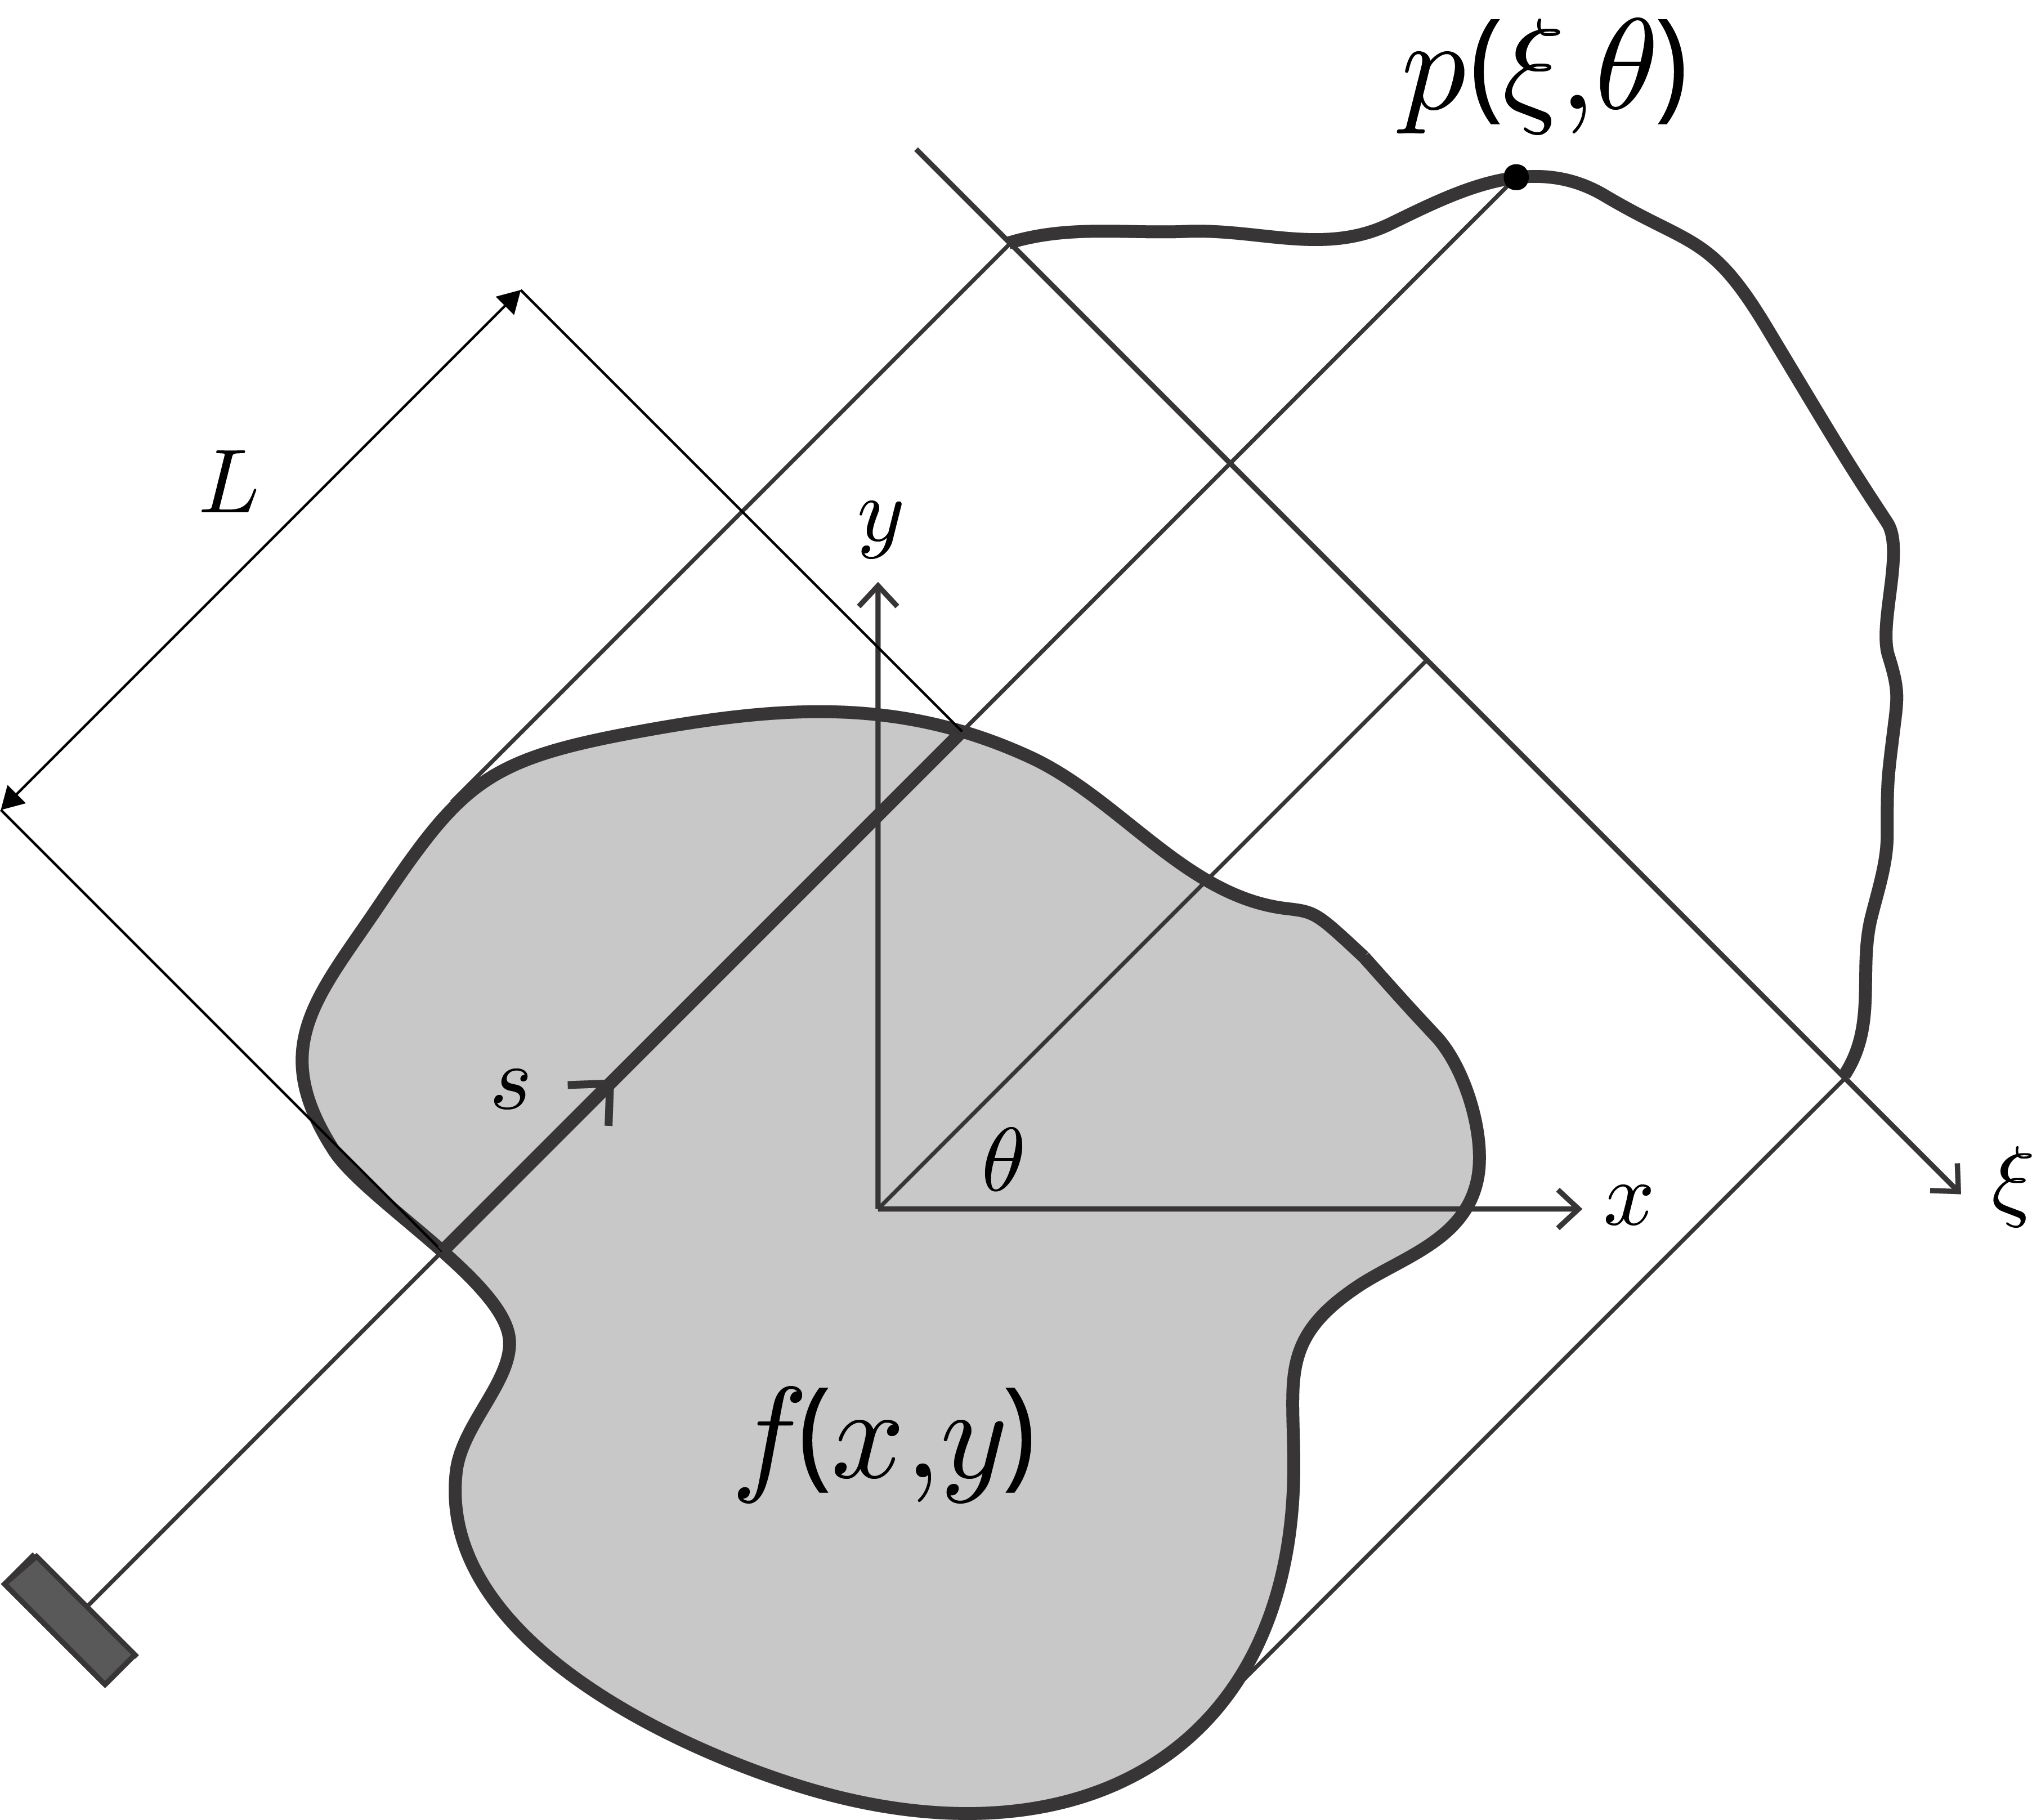
\includegraphics[scale=0.3]{media/0-imaging/ct3.png}
%
\caption{Linear attenuation function $f(x,y)$ for a particular slice, and corresponding projection $p(\xi,\theta)$}
\label{fig:ct3}
\end{figure}

The function $p$ for each $\theta$ view is known as a \textit{projection} of the image $f$. The most popular image reconstruction technique is \textit{backprojection}, in which the function $f$ is computed from the projections $p$. Backprojection leads to a blurring of the original image, so the projected images are first filtered prior to backprojection. The total technique is known as \textit{filtered backprojection}. The Fourier transform of $p$ is computed, a ramp filter is applied in frequency space, the inverse Fourier transform of the resulting function is computed, and finally the inverse Radon transform is applied to approximate $f(x,y)$. Filtered backprojection performs best in the presence of a large number of projections, which is the case in modern CT scanners. A more detailed description of the procedure is provided by Chetih \textit{et al.}~\cite{chetih_2015}.

Finally, the value computed at each voxel is rescaled to produce the \textit{CT number}. The CT number is defined as $K (f_i - f_w)/f_w$, measured in \textit{Hounsfield units}. The scaling parameter $K$ is typically a value of 1000 in modern machines. The value $f_i$ is the attenuation at a particular voxel, and the value $f_w$ is the attenuation of water. The attenuation coefficient of water is obtained during calibration of the machine.

Improvements in acquisition times, spatial resolution, and image reconstruction times have been made in the last 45 years since the first-generation CT machine was introduced. These improvements mostly involve an increase in x-ray detectors and more clever arrangements and motions of the x-ray beam and associated detector(s). Detailed descriptions of these improvements can be found in the references cited in this section.

\subsection{Additional Imaging Modalities}
\label{Other Imaging Modalities}

Several other popular imaging modalities exist in addition to MRI and CT. The discussion here will be restricted to a brief overview of \textit{ultrasound} (US), as well as some quantitative variations of MRI, CT, and US.

Ultrasound uses high-frequency sound pulses that are emitted from a hand-held ultrasound transducer~\cite{waldman_campbell}. The transducer is applied to the patient's skin through a coupling gel, and sound pulses are reflected back to the transducer from structures within the patient. The magnitude of the reflected sound, or \textit{echo}, is converted into a 2D grayscale image. Images are acquired in real-time, and do not require any ionizing radiation. Ultrasound is most commonly used for imaging the abdominal and pelvic regions, as well as imaging the musculoskeletal system. When used to image the heart, ultrasound is referred to as \textit{echocardiography}. Three-dimensional ultrasound techniques have been gaining traction in recent decades, of which there are two varieties for 3D reconstruction: random or \textit{freehand scanning} which is based on free motion of the ultrasound transducer; and \textit{sequential scanning} where the ultrasound motion is predetermined in linear, fan-like or rotational patterns~\cite{valocik_2005, bruining_2000}.

Quantitative versions of the modalities discussed attempt to extract material property information in addition to only contrasting different tissues. \textit{Diffusion-tensor imaging} (DTMRI) is used to measure the anisotropy of tissues. Additional magnetic field gradients are applied repeatedly to create images that are sensitized to the diffusion of water in specific directions~\cite{o'donnell_westin_2011}. The diffusivity tensor is approximated at each voxel, and may be used to visualize irregularities in the microstructure of the brain~\cite{alexander_lee_lazar_field_2007}, or to approximate cardiac muscle fiber orientations. \textit{Elastography} is the process of quantitatively imaging the mechanical properties of soft tissues \textit{in vivo}, and is performed using either magnetic resonance or ultrasound techniques~\cite{zaleska_2014}. The process involves first applying a stress or source of motion that deforms the tissue, next imaging the tissue response, and finally processing the data to generate images (\textit{elastograms}) of tissue mechanical properties~\cite{glaser_manduca_ehman_2012}. \textit{Quantitative computed tomography} (QCT) estimates bone mineral density from CT attenuation data by using a calibration phantom during image acquisition. This information can be used to inform heterogeneous material definitions in computational models of bone~\cite{knowles_2016}.

A more complete review of medical imaging technologies can be found in a number of texts~\cite{webb_2003, suetens_2017}.

\subsection{File Formats}
\label{Data Format-IMG}

Medical images are typically stored as a combination of a short \textit{header} followed by \textit{voxel data}. The header is typically stored in ASCII format and the voxel data is typically binary. They may be found in the same file or in separate ones. Voxel data is often stored either as a set of two-dimensional images representing each slice, or as a single block of information corresponding to the 3D volume. In either case, data is stored as a 1D array, from which the data can be unrolled based on the axis ordering specified in the header. The header provides metadata to allow software to read and store the image based on the voxel data. Namely, the header contains the matrix dimensions, image resolution, image origin, axis order, data type of the voxel data (i.e., \texttt{unsigned char}, \texttt{int}, etc.), endianness of the voxel data, and data compression encoding (e.g., raw, gzip, bzip2). Additional information may be provided as well, including patient data, image acquisition parameters (e.g., MRI pulse sequence), and date of acquisition. On the clinical side, DICOM (Digital Imaging and Communications in Medicine) files are by far the most popular format for storing medical images, due to it's extensive metadata including patient information and image acquisition protocol. Several formats are available in research, including MATLAB~\cite{MATLAB}, NRRD (Nearly Raw Raster Data)~\cite{nrrd}, NIfTI (Neuroimaging Informatics Technology Initiative)~\cite{nifti}, and Analyze~\cite{analyze}. These file formats are different flavors of the same general format described above. By containing less detailed and cumbersome metadata sections, they are geared more towards image post-processing compared to DICOM.

%%%%%%%%%%%%%%%%%%%%%%%%%%%%%%%%%%%%%%%%%%%%%%%
%%%%%%%%%%%%%%%%%%%%%%%%%%%%%%%%%%%%%%%%%%%%%%%
\section{Image Segmentation Approaches}
\label{Image Segmentation Approaches}

Arguably the most challenging step in producing a robust workflow is the subsequent processing and segmenting of the image of interest. \textit{Image segmentation} is the process of partitioning an image into non-overlapping regions corresponding to different tissues or objects in an image. Contrast differences between neighboring tissues can be difficult to identify, and thus \textit{image processing} is first performed.

\subsection{Image Processing}
\label{Image Processing}
In image processing, filters are applied to the image to alter voxel intensity values, which can remove noise and emphasize features of the image so as to improve the performance of image segmentation algorithms. Processing the image data begins with \textit{resampling}. Images almost always have a higher resolution in-plane than in the slice direction. Segmentation techniques typically prefer \textit{isotropic voxel spacing}, meaning the resolution of the image is the same in all three directions. Thus, images are resampled such that isotropic voxel spacing is achieved. Resampling simply involves interpolating voxel data from the original coarser image to the new voxel locations of the artificially finer resampled image. Any number of interpolation bases may be used, but practically speaking the basis choice is insignificant for images with clinical resolutions, and can be as simple as linear interpolation.

The image is additionally processed to remove noise and artifacts, as well as to emphasize tissue interfaces for more successful application of image segmentation techniques. Image filters include the \textit{Gaussian blur filter}, \textit{mean filter}, and \textit{median filter}~\cite{Seg3D}. Each of these are known as smoothing filters, but in fact facilitate the identification of tissue interfaces by producing larger regions of more homogeneous voxel intensities. The median filter is particularly effective in reducing the \textit{salt and pepper sign} commonly found in MRI, in which tissues have a speckled appearance.

\subsection{Review of Image Segmentation Approaches}
\label{Review of Image Segmentation Approaches}

Following resampling and processing, image segmentation is performed to identify the tissues and objects of interest. If the domain of the image is given by $\Omega$, the segmentation problem is to determine the sets $S_k \subset \Omega$, such that:
\begin{align}
\Omega &= \bigcup \limits_{k=1}^{K} S_k \\
S_k \cap S_j &= \emptyset, \text{\ \ } k \neq j
\end{align}
where $K$ is the total number of classifications in the image. Often, the value of K is assumed to be known based on prior knowledge of the anatomy being considered~\cite{pham_2000}. Each voxel in the image is assigned a tag corresponding to the region to which it belongs, resulting in what is known as an \textit{image mask}. The image and resulting and image mask are shown in~\figref{seg} for an \textit{ex vivo} MRI of a human heart from the CardioVascular Research Grid~\cite{cvgg}. An enormous number of image segmentation techniques exist in the literature; a few popular techniques are mentioned here.

\begin{figure}[ht]
\centering
\subfigure[]{%
		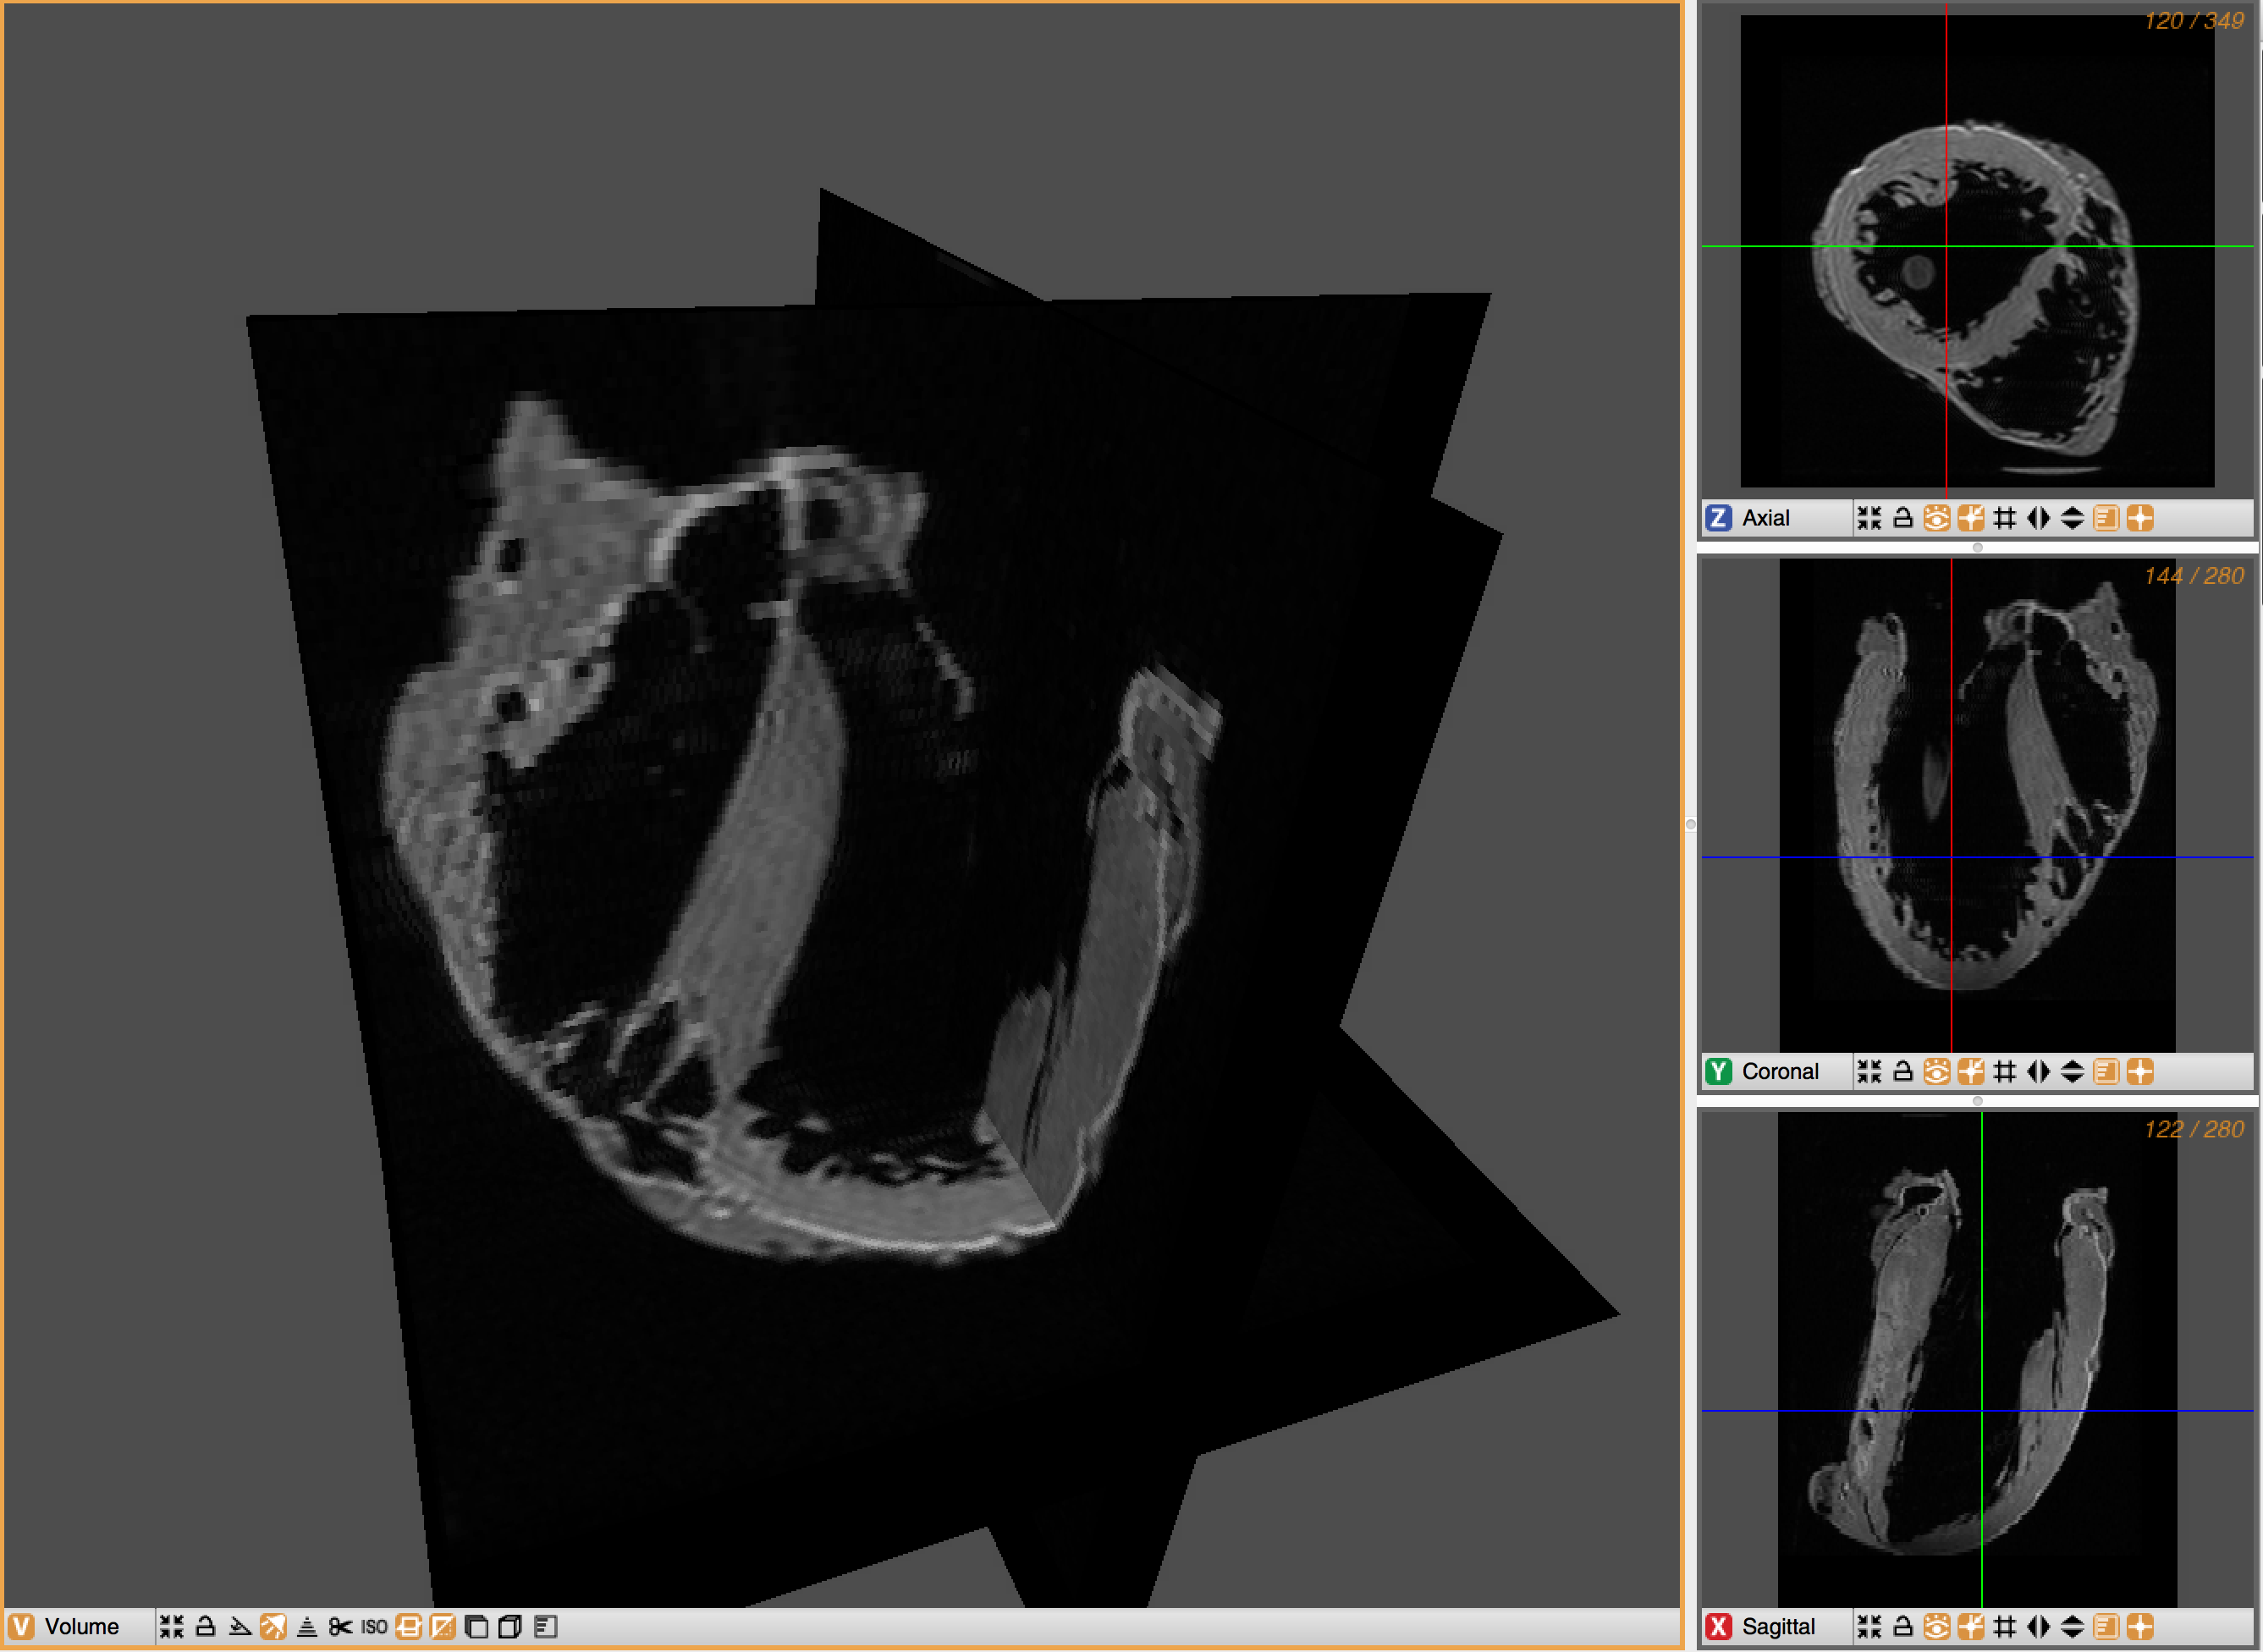
\includegraphics[scale=0.165]{media/1-seg3d/1-raw.png}
\label{fig:seg1}}
\subfigure[]{%
		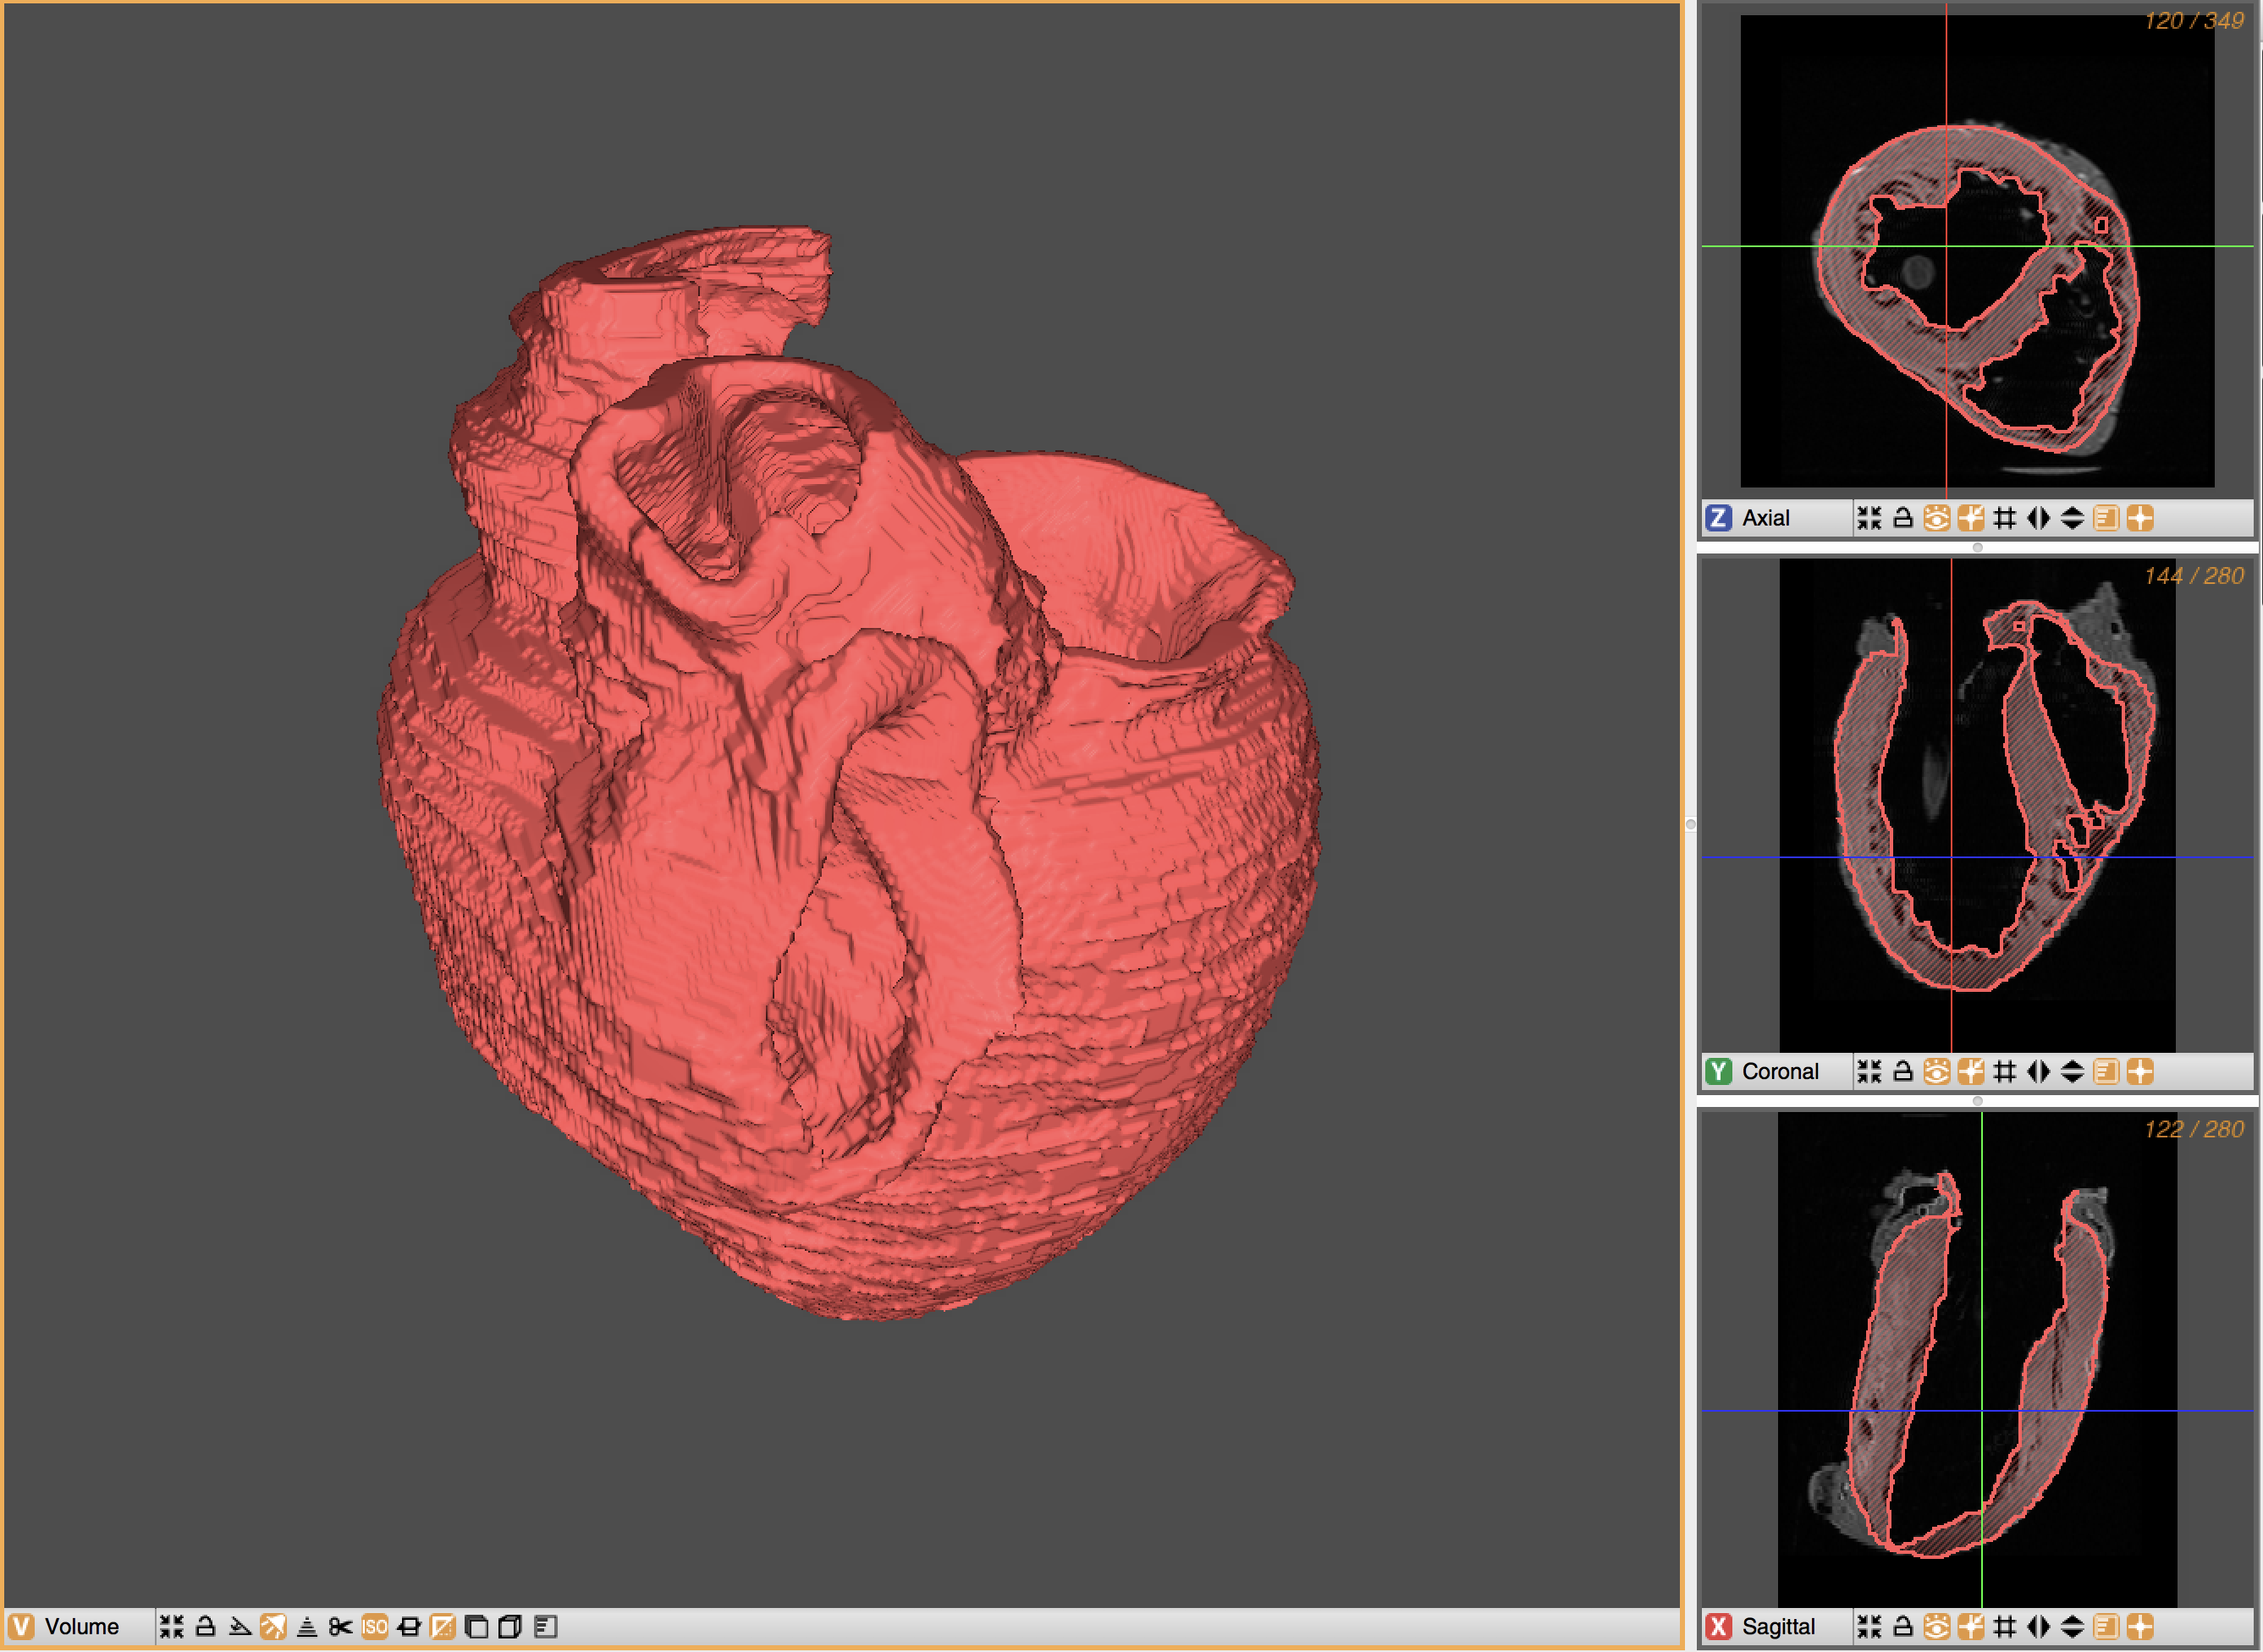
\includegraphics[scale=0.165]{media/1-seg3d/2-seg.png}
\label{fig:seg2}}
%
\caption{(a) MRI of \textit{ex vivo} human heart, and (b) resulting segmented image mask}
\label{fig:seg}
\end{figure}

\textit{Thresholding} delineates images based on voxel intensities alone. A thresholding procedure attempts to determine the intensity value - the threshold - that separates two different regions. A histogram of image intensities may have several modes depending on the number of regions $K$, though, so several thresholds are generally applied (known as \textit{multithresholding}). These threshold values are selected based on the local minima present in the intensity histogram. Thresholding is often performed interactively, based on the operator's visual assessment of the resulting segmentation. It does not take into account the spatial characteristics of an image, which causes it to be sensitive to noise and intensity inhomogeneities. \textit{Region-based segmentation} merges or splits regions of voxels based on whether they share homogeneity criteria. \textit{Edge detection techniques} determine the edges of distinct regions based on gradients of the image intensity. Edge detection is not on its own a segmentation technique, but rather must be used in conjunction with region-based approaches to generate a segmentation. For example, following edge detection, a seed of voxels may be grown until the edges are reached.

\textit{Deformable models} use parametric surfaces that deform under the influence of artificial internal and external forces relating to characteristics of the image. A seed surface is initiated by the user, followed by an iterative process in which the surface deforms to the shape of the interface in the image. Internal forces aim to keep the surface smooth during deformation, and external forces drive the surface toward the desired shape. A particularly well known and effective set of approaches are \textit{level set methods}. In these approaches, a level set surface $\phi$ begins as a signed distance function $d(\bm{x})$ from the seed surface and evolves toward the desired surface with a speed whose normal component is $F$. The \textit{level set equation} is an advection equation that has the following form:
\begin{align}
\frac{\partial \phi}{\partial t} + F \left| \nabla \phi \right| = 0 \\
\phi(t=0) = d(\bm{x})
\end{align}
The front speed $F(\bm{x})$ depends on the gradient of image intensity and the curvature of the surface. This advection equation is solved using ordered upwind methods, most notably the \textit{fast marching method}~\cite{malladi_1995, sethian_1996}. The converged solution is the resultant surface for which $d = 0$. Being an implicit function, it must still be converted to an explicitly defined image mask, in the same way that edge detection methods rely on region-based methods.

\textit{Atlas guided approaches} treat segmentation as a \textit{registration} problem in which a presegmented atlas (or template) image is transformed to a target image requiring segmentation. Atlas-guided approaches are best suited for segmentation of structures that are stable over the population of the study, and may require manual selection of landmarks to constrain the nonlinear registration process. \textit{Machine learning methods} make use of \textit{neural networks} in which a set of weights associated with the nodes in a learning network are adapted based on \textit{training data}. See Litjens \textit{et al.} for a detailed description~\cite{litjens_2017}.

Many other image segmentation techniques exist, including \textit{classifier methods} and \textit{clustering methods}. The literature referenced in this section provide a detailed description of these other techniques.

Practically speaking, image segmentation algorithms to date are not typically robust enough for automated general purpose applications. In almost all cases, manual interaction and/or post-processing are required or at least preferable. Human intervention can unfortunately be laborious and time-consuming, though, and raises reliability issues for large population studies. Additionally, segmentations are typically most effective when multiple algorithms are used in conjunction with one another. For example, an image mask generated by thresholding is a an effective initial seed to region-based and deformable model approaches. Commercial and free software with graphical user interfaces (GUIs) significantly facilitate using multiple segmentation techniques, not the least of which manual fine-tuning techniques such as \textit{paintbrush} tools. Of the most popular tools available are OsiriX, Simpleware, Mimics, and Seg3D. Producing accurate image masks in a timely manner is to date still as much an art as it is a science.

\subsection{File Formats}
\label{Data Format-SEG}

Image masks are typically stored in the same format as the image data themselves, as described previously. The data at each entry in the matrix is simply an unsigned integer corresponding to the region to which the voxel belongs. The background, also referred to as \textit{void}, is assigned a value of 0. Image masks of a single tissue or object are known as \textit{binary masks}, for which voxel entries only have values of 0 for void or 1 for the tissue of interest.
